\question 有效地址是指( )
\par\twoch{\textcolor{red}{操作数的真实地址}}{指令地址码字段给出的地址}{程序计数器(PC)给出的地址}{以上均不正确}
\begin{solution}本题考查有效地址的概念。有效地址就是操作数的真实地址。指令地址码字段给出的地址可能是有效地址,也可能不是,统称为形式地址。程序计数器(PC)给出的是下一条即将执行指令的地址(当然这句话不够严谨,也可以程序计数器(PC)给出的是当前正在执行指令的地址,但是这些都不是重点,等学完有关CPU章节后会明白为什么两者说法都对,但一般都是指下一条即将执行指令的地址)。
\end{solution}
\question 下列关于指令字长、机器字长和存储字长的说法中,正确的是
Ⅰ.指令字长等于机器字长的前提下,取指周期等于机器周期
Ⅱ.指令字长等于存储字长的前提下,取指周期等于机器周期
Ⅲ.指令字长和机器字长的长度没有必然关系
Ⅳ.为了硬件设计方便,指令字长都和存储字长一样大
\par\twoch{Ⅰ、Ⅲ和Ⅳ}{Ⅰ和Ⅳ}{\textcolor{red}{Ⅱ和Ⅲ}}{Ⅱ、Ⅲ和Ⅳ}
\begin{solution}C。
指令字长是指指令中包含二进制代码的位数;机器字长是CPU一次能处理的数据长度,通常等于内部寄存器的位数;存储字长是一个存储单元存储的二进制代码(存储字)的长度。
指令字长通常都是取存储字长的整数倍,如果指令字长等于存储字长的2倍,则需要2次访存,那么取指周期就等于机器周期的2倍;如果指令字长等于存储字长,那么取指周期就等于机器周期,故Ⅰ错误、Ⅱ正确。指令字长取决于操作码的长度、操作数地址的长度和操作数地址的个数,与机器字长没有必然的联系,但为了硬件设计方便,指令字长一般取字节或存储字长的整数倍,故Ⅲ正确。指令字长一般取字节或存储字长的整数倍,而不一定都是和存储字长一样大,故Ⅳ错误。
\end{solution}
\question (西安理工大学,2002年)二地址指令中,操作数的物理位置不可安排在
\par\twoch{\textcolor{red}{栈顶和次栈顶}}{两个主存单元}{一个主存单元和一个寄存器}{两个寄存器}
\begin{solution}A。
二地址指令有两个操作数,这些操作数并不一定都在主存中,往往有一个或两个在通用寄存器中,这样就构成了不同的类型。下面介绍不同二地址指令的区别,见下表:
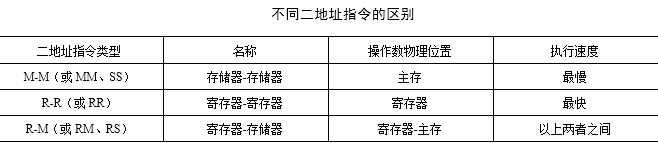
\includegraphics[width=6.85417in,height=1.48958in]{computerassets/4816e952d855fb6bd05b9a469095a3a0.jpeg}
\end{solution}
\question (北京理工大学,2002年)在一地址格式的指令中,下列( )是正确的
\par\fourch{仅有一个操作数,其地址由指令的地址码提供}{\textcolor{red}{可能有一个操作数,也可能有两个操作数}}{一定有两个操作数,另一个是隐含的}{以上都不对}
\begin{solution}B。 一地址指令一般分为两种:
(1)只有目的操作数的单操作数指令,按A地址读取操作数,进行OP操作后,结果存回原地址。例如,操作码含义是加1、减1、求反、求补等。
(2)隐含约定目的地址的双操作数指令。按指令地址A可读取源操作数,指令可隐含约定另一个操作数由AC提供,运算结果也将存放在AC中。
综上分析,一地址格式的指令中,可能有一个操作数,也可能有两个操作数。
\end{solution}
\question (北京理工大学,2002年)在二地址指令中,( )是正确的
\par\fourch{指令的地址码字段存放的一定是操作数}{指令的地址码字段存放的一定是操作数地址}{\textcolor{red}{运算结果通常存放在其中一个地址码所提供的地址中}}{指令的地址码字段存放的一定是操作码}
\begin{solution}C。
指令的地址码存放的可能是操作数(立即寻址),也可能是操作数地址(直接寻址)。故选项A和B错误。选项D明显错误,操作码存放在操作码字段中。
\end{solution}
\question 关于单地址指令,下列说法正确的是
\par\twoch{只能对单操作数进行加工处理}{只能对双操作数进行加工处理}{无处理双操作数的功能}{\textcolor{red}{既能对单操作数进行加工处理,也能对双操作数进行运算}}
\begin{solution}D。
单地址指令可以实现单操作数指令也实现完成双操作数指令,单操作数指令很好理解,单地址对应单操作数。对于双操作数的情况,一般单地址对应一个操作数,另一个操作数隐藏在运算器的ACC中。
\end{solution}
\question 在通用计算机指令系统的二地址指令中,操作数的物理位置可安排在
Ⅰ.一个主存单元和缓冲存储器 Ⅱ.两个数据寄存器
Ⅲ.一个主存单位和一个数据寄存器 Ⅳ.一个数据寄存器和一个控制存储器
Ⅴ.一个主存单元和一个外存单元
\par\twoch{Ⅱ、Ⅲ和Ⅳ}{\textcolor{red}{Ⅱ和Ⅲ}}{Ⅰ、Ⅱ和Ⅲ}{Ⅰ、Ⅱ、Ⅲ和Ⅴ}
\begin{solution}B。
对于二地址指令,若两个操作数都在寄存器中,称为RR型指令;若一个操作数在寄存器中另一个操作数在存储器中,称为RS型指令;若两个操作数都在存储器中,则称为SS型指令。(一般用R表示寄存器,S表示存储器)RR型执行速度最快,SS型执行速度最慢,RS型执行速度介于RR型和SS型之间。
缓冲存储器(如Cache),用来存放最近使用的数据,其内容和调度都是由硬件或操作系统完成的,因此不能作为指令的地址码。控制存储器采用ROM结构,存放的是微程序,它对软件开发人员是透明的,显然不能作为指令的地址码。CPU不能直接访问外存,如果所需的数据存放在外存,则需要先调入主存,而指令中只能使用主存地址。
\end{solution}
\question 下述关于零地址指令的说法正确的是
\par\fourch{零地址指令是不需要操作数的指令}{零地址指令需要有操作数,其操作数通过隐含寻址得到}{\textcolor{red}{有的零地址指令不需要操作数,有的零地址指令需要并使用隐含寻址得到操作数}}{以上说法都不正确}
\begin{solution}C。
在知识点讲解中详细讲到,有些零地址指令是不需要操作数的,如停机指令;有些零地址指令需要操作数,其操作数通过隐含寻址得到,即其操作数来自于栈顶和次栈顶。
\end{solution}
\question 零地址双操作数指令不需要指出操作数地址,这是因为
\par\twoch{操作数已在数据缓冲寄存器中}{操作数隐含在累加器中}{\textcolor{red}{操作数地址隐含在堆栈指针中}}{利用上一条指令的运算结果进行操作}
\begin{solution}C。
零地址运算指令在指令格式中不给出操作数的地址,它的操作数来自栈顶和次栈顶。
\end{solution}
\question 二地址指令中,操作数的物理位置可安排在 Ⅰ.两个主存单元 Ⅱ.两个寄存器
Ⅲ.一个主存单元和一个寄存器
\par\twoch{Ⅰ、Ⅱ}{Ⅱ、Ⅲ}{Ⅰ、Ⅲ}{\textcolor{red}{Ⅰ、Ⅱ、Ⅲ}}
\begin{solution}D。 二地址指令的两个操作数位置可以在寄存器和主存中随便选择位置存放。
\end{solution}
\question 四地址指令OP A1 A2 A3
A4的功能为(A1)OP(A2)→A3,且A4给出下一条指令地址,假设A1、A2、A3、A4都为主存储器地址,则完成上述指令需要访存(
)次
\par\twoch{2}{3}{\textcolor{red}{4}}{5}
\begin{solution}C。
首先取指令需要1次访存(不少考生会忽略),然后取两个操作数两次访存,保存运算结果1次访存,一共需要4次访存。
\end{solution}
\question (国防科技大学,2003年)设指令中的地址码为A,变址寄存器为X,程序计数器为PC,则变址寻址方式的操作数的有效地址为
\par\twoch{(PC)+A}{(A)+(X)}{(A+X)}{\textcolor{red}{A+(X)}}
\begin{solution}D。
变址寻址的指令是将规定的变址寄存器中的内容加上指令中给出的偏移量,就可得出操作数的有效地址。
\end{solution}
\question (武汉大学,2007年)指令``MOV
AX(源地址),{[}BX+SI{]}(目的地址)''的源操作数的寻址方式是
\par\twoch{\textcolor{red}{寄存器寻址}}{寄存器间接寻址}{变址寻址}{基址寻址}
\begin{solution}A。
源操作数存放在寄存器AX中,故为寄存器寻址;如果是(AX)就是寄存器间接寻址。
\end{solution}
\question (西安电子科技大学,2007年)在指令的相对寻址方式中,其相对的基准地址是
\par\twoch{基址寄存器}{变址寄存器}{堆栈指示器}{\textcolor{red}{程序计数器}}
\begin{solution}D。
相对寻址是把程序计数器(PC)的内容加上指令格式中的形式地址而形成操作数的有效地址,即EA=(PC)+A,故基准地址是程序计数器。
\end{solution}
\question (中科院算计所,2000年)( )寻址方式用来支持浮动程序设计
\par\twoch{\textcolor{red}{相对寻址}}{变址寻址}{寄存器间接寻址}{基址寻址}
\begin{solution}A。 参考下表:
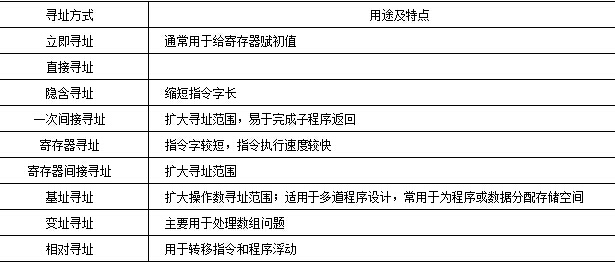
\includegraphics[width=6.40625in,height=2.73958in]{computerassets/250008b810db3ded5679f33d4628c374.jpeg}
\end{solution}
\question (西南交通大学,2005年)在下面几种寻址方式中,( )方式取操作数最快
\par\twoch{直接寻址}{\textcolor{red}{寄存器寻址}}{相对寻址}{变址寻址}
\begin{solution}B。
A选项的操作数在主存中,需要访问一次主存;B选项只需要访问一次寄存器;C和D选项首先要进行加法运算,再访问主存。所以寄存器寻址方式取操作数是最快的。
\end{solution}
\question 在下列寻址方式中,( )方式需要先计算,再访问主存
\par\twoch{相对寻址}{变址寻址}{间接寻址}{\textcolor{red}{A和B}}
\begin{solution}D。
相对寻址:相对寻址的有效地址是将程序计数器PC的内容与指令字中的形式地址A相加而成。相对寻址的有效地址为EA=(PC)+A。
变址寻址:指令指定一个CPU寄存器(称为变址寄存器)和一个形式地址,操作数地址是二者之和,需要先计算再访存。变址寻址的有效地址为EA=A+(IX)。
间接寻址:指令给出存放操作数地址的存储单元地址,先得到操作数地址所在的存储单元的地址,再得到操作数的地址,然后才能取操作数。
所以A和B都是符合的,选D。
\end{solution}
\question 以下说法中正确的是
\par\fourch{寻址方式是指令如何给出操作数或操作数地址}{所有指令的寻址方式都相同}{所有指令都有操作码和地址码}{\textcolor{red}{指令的功能与寻址方式无关}}
\begin{solution}D。
寻址方式是处理器根据指令中给出的地址信息来寻找物理地址的方式,与指令的功能无关。
\end{solution}
\question 一个较完善的指令系统应包含运算类、数据传送类、控制类、( )等指令
\par\twoch{\textcolor{red}{I/O}}{栈操作}{子程序调用}{条件转移}
\begin{solution}A。
正确答案是I/O类指令。本题可用排除法:栈操作可归到数据传送类指令,条件转移可归到控制类指令,子程序调用就是转移指令,属控制类指令。
\end{solution}
\question 执行for循环时,需要传送循环次数值给某专用寄存器,一般使用的寻址方式是
\par\twoch{\textcolor{red}{立即寻址}}{直接寻址}{基址寻址}{相对寻址}
\begin{solution}A。
立即寻址用途一:例如需要传送一个循环次数给某专用寄存器(比如for循环的循环次数),则可以使用立即寻址直接将循环次数作为立即数送入。
立即寻址用途二:例如需要将某程序的首地址送入PC(程序计数器)中,而程序的首地址可以看成是一个操作数,则可以使用立即寻址直接将该程序的首地址作为立即数送入。
用途总结:立即数寻址方式通常用于对某寄存器或内存单元赋初值。
\end{solution}
\question 若变址寄存器编号为X,形式地址为D,则变址寻址方式的有效地址为
\par\twoch{\textcolor{red}{R[X]+D}}{R[X]+[D]}{M[R[X]+D]}{M[R[X]+[D]]}
\begin{solution}A。 九种寻址方式总结如下表所示:
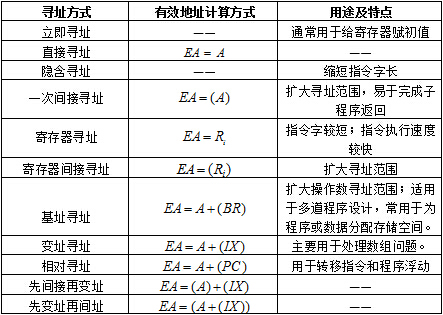
\includegraphics[width=4.61458in,height=3.28125in]{computerassets/87b5c054d339fca75d9d85ad9c016aff.jpeg}
\end{solution}
\question 假设某指令的一个操作数采用变址寻址方式,变址寄存器中的值为007CH,地址007CH中的内容为0124H,指令中给出的形式地址为B000H,地址B000H中的内容为C000H,则该操作数的有效地址为
\par\twoch{B124H}{C124H}{\textcolor{red}{B07CH}}{C07CH}
\begin{solution}C。
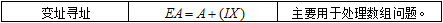
\includegraphics[width=4.61458in,height=0.23958in]{computerassets/42915143abc5fc9d27b6626825afca7e.jpeg}
依题意,A=B000H,(LX)=007CH,那么EA=B000H+007CH=B07CH。
\end{solution}
\question 某计算机字长32位,CPU中有32个32位通用寄存器,采用单字长定长指令字格式,操作码占6位,其中还包含对寻址方式的指定。对于存储器直接寻址方式的RS型指令,能直接寻址的最大地址空间大小是
\par\twoch{\textcolor{red}{$2^21$}}{$2^26$}{$2^27$}{$2^32$}
\begin{solution}A。
因为有32个通用寄存器,所以寄存器编号为5位。存储器直接寻址的RS型指令的一个操作数在寄存器中,所以指令中必须有一个5位的寄存器编号,另外一个地址码是直接地址,共有32-6-5=21位。指令格式如下图所示:
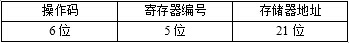
\includegraphics[width=3.63542in,height=0.44792in]{computerassets/f59d9d0e012ea401c6f7b94b23fae953.jpeg}
所以,能直接寻址的最大地址空间大小是2\^{}21。
\end{solution}
\question 一般来说变址寻址经常和其他寻址方式混合在一起使用,设变址寄存器为IX,形式地址为D,某机具有先间址寻址再变址寻址的方式,则这种寻址方式的有效地址为
\par\twoch{EA=D+(IX)}{\textcolor{red}{EA=(D)+(IX)}}{EA=(D+(IX))}{EA=D+IX}
\begin{solution}B。
先间址后变址,这里需要理清``先间址''的这个间址指的是D,而不是IX,如果是IX的话那就变成了寄存器间接寻址了。
这里先把寄存器单元内容当作地址,再加上形式地址(D)得到操作数的地址,即EA=(D)+(IX),所以正确答案是B。
如果本题改为先变址寻址再间接寻址的方式,答案应该是EA=(D+(IX))。
这里的先后指的是表达式的先后计算顺序,记住这点,就不会出错了。比如EA=(D)+(IX)这个表达式,需要先求(D)即先间址。而EA=(D+(IX))这个表达式,需要先求D+(IX)即先变址。
知识点回顾:
变址寻址的有效地址EA=A+(IX),其中A为形式地址,IX为变址寄存器。
变址寻址中,变址寄存器的内容是由用户设定的,在程序执行过程中其值可变,而指令字中的形式地址A是不可变的。这点恰好和基址寄存器相反。
\end{solution}
\question 间址寻址第一次访问内存所得到信息经系统总线的( )传送到CPU
\par\twoch{\textcolor{red}{数据总线}}{地址总线}{控制总线}{总线控制器}
\begin{solution}A。
系统总线按传送内容的不同可分为地址总线、数据总线和控制总线。地址总线由单向多根信号线组成,可用于CPU向主存、外设传送地址信息;数据总线由双向的多根信号线组成,CPU可以沿着这些线从主存或外设读入数据,也可发送数据;控制总线上传输控制信息,包括控制命令和反馈信号等。
间址寻址第一次访问内存所得到的信息是操作数的有效地址,该地址通过数据线传送至CPU而不是地址线。地址线是单向总线,只能由CPU向主存和外设传送。
\end{solution}
\question 下列关于各种寻址方式获取操作数快慢的说法中,正确的是
Ⅰ.立即寻址快于堆栈寻址 Ⅱ.堆栈寻址快于寄存器寻址
Ⅲ.寄存器一次间接寻址快于变址寻址 Ⅳ.变址寻址快于一次间接寻址
\par\twoch{Ⅰ和Ⅳ}{Ⅱ和Ⅲ}{\textcolor{red}{Ⅰ、Ⅲ和Ⅳ}}{Ⅲ和Ⅳ}
\begin{solution}C。
因为访问寄存器的速度通常是访问主存的数十倍,所以获取操作数快慢主要取决于寻址方式的访存次数。
立即寻址操作数在指令中,不需要任何访问寄存器或内存,取数最快,Ⅰ正确。堆栈寻址可能是硬堆栈(寄存器)或软堆栈(内存),采用软堆栈时比寄存器寻址慢,Ⅱ错误。寄存器一次间接寻址先访问寄存器得到地址,然后再访问主存;而变址寻址访问寄存器IX后,还要将A和(IX)相加(相加需要消耗时间),再根据相加的结果访存,显然后者要慢一点,Ⅲ正确。一次间接寻址需要两次访存,显然慢于变址寻址,Ⅳ正确。
\end{solution}
\question 设相对寻址的转移指令占两个字节,第一个字节是操作码,第二个字节是相对位移量(用补码表示),若CPU每当从存储器取出一个字节时,即自动完成(PC)+1→PC。若当前PC的内容为2008H,要求转移到2001H,则该转移指令第二字节的内容为
\par\twoch{05H}{07H}{F8H}{\textcolor{red}{F7H}}
\begin{solution}D。
相对寻址的形式地址中存放的是相对位移量。有效地址是将PC的内容加上指令格式中的形式地址A的结果。
由于转移指令占两个字节,当前PC的内容为2008H,取出第一字节的操作码后,PC的内容为2009H,取出第二字节的位移量后,PC的内容为200AH,因此,在执行该转移指令计算转移目标地址时,PC已经是200AH了。因为转移目标为2001H,所以此时的位移量是2001H-200AH=-9H,用补码表示为F7H。
\end{solution}
\question CPU内有32个32位的通用寄存器,设计一种能容纳64种操作的指令系统。假设指令字长等于机器字长,如果主存可直接或间接寻址,采用``寄存器---存储器''型指令,采用通用寄存器作基址寄存器,能直接寻址的最大存储空间是
\par\twoch{\textcolor{red}{4G}}{64M}{2M}{1M}
\begin{solution}A。
如采用基址寻址,则指令格式中应给出基址寄存器号,以指定哪一个通用寄存器用作基址寄存器。指令格式如下图所示:
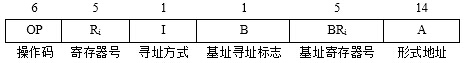
\includegraphics[width=4.84375in,height=0.65625in]{computerassets/7abb2d9c3bbfc12cb302dfa8413e1155.jpeg}
寻址的最大空间=2\^{}32=4G字,其寻址范围仅与基址寄存器位数有关,与形式地址位数无关。
\end{solution}
\question 寄存器中的值可能是地址,也可能是数据,它们的内容本身没有区别,计算机需要识别它是数据还是地址,是根据
\par\twoch{寄存器编号}{判断程序}{\textcolor{red}{指令操作码或寻址方式位}}{时序信号}
\begin{solution}C。
有的同学可能会选A,举出的特例是MAR存的就是地址,MDR存的就是数据。首先我们要区分下地址和数据,当我们用这个内容用来寻址的时候,那它就是地址,当我们用这个内容进行运算的时候它就是数据。所以内容上没有一个本质的区别,只有用的时候才知道它是地址还是数据,故本题应该选C。
\end{solution}
